\chapter{Particle Accelerator Physics}\label{chap:2}
%
\section*{Introduction}
%
The history of particle accelerators goes back to the 1930s when the first accelerators were designed to provide the particle energies required to study atomic nuclei. Nowadays, a vast variety of accelerator types is available for many different applications, reaching from low-energy machines for particle therapy in cancer treatment (for example Heidelberger Ionenstrahl-Therapiezentrum, HIT~\cite{HITref01}) over synchrotron light sources at intermediate energies (for example SOLEIL~\cite{SOLEILref01}) to high-energy synchrotron colliders for fundamental research, such as the Large Hadron Collider, presented in \chapref{thelhc}.

This chapter gives an overview of physics aspects in modern hadron synchrotrons. The first section demonstrates the general description of essential beam properties, such as the transverse and longitudinal beam behaviour in the magnetic lattice of an accelerator. The focus is set to the functionality of the different elements used in the accelerator, considering particles of a defined species. The second section presents the theoretical description of the particle movement of arbitary particles in the magnetic lattice by means of the Hamiltonian formalism. 
%

\section{Particle Dynamics in Electromagnetic Fields}

\subsection{Reference frame} \label{chap:refframe}


\input{pictures/refframe.tex}



Particle beams in circular accelerators are bent by means of magnetic dipole fields. With the design of the machine, a closed reference trajectory is defined which leads typically through the center of the beam pipes and magnets. This trajectory corresponds to the orbit of a particle at design momentum without transverse offsets, which is referred to as the ideal particle. With respect to the curvlinear laboratory frame ($\hat X, \hat Y, \hat Z$), the position of the reference particle at the time $t$ is defined by the vector $\textbf{r}(s)$, where $s(t)$ is a parameter describing the distance travelled from a defined reference point in the accelerator (see \figref{fig:frame}). The cartesian accelerator coordinate system ($\hat x, \hat y, \hat z$), spanned by the unitary vectors ($\textbf{e}_x, \textbf{e}_y, \textbf{e}_z$), moves with the reference particle and thus with $\textbf{r}(s)$, as shown in \figref{fig:frame}. The particle position in the laboratory frame is then fully characterized by the vector
%
\begin{align}
\textbf{Q}(x,y,z,s) = \textbf{r} (s) + x  \, \textbf{e}_x + y \,  \textbf{e}_y + z \, \textbf{e}_z \, . \label{eq:refframe}
\end{align}
%
Inside the dipole magnets, the trajectory of the vector $\textbf{r}(s)$ is bent by a radius 
\begin{align}
\rho = \frac{1}{h_x} \, .
\end{align}
%
%%
%
Electromagnetic fields are generally defined by the gradient of the electric scalar potential $V$ and the magnetic vector potential $\textbf{A}$. In the curvliniar reference system $(x,y,s,t)$, spanned by the unitary vectors $(\textbf{e}_x,\textbf{e}_y,\textbf{e}_s)$, the electromagnetic fields $\textbf{E}$ and $\textbf{B}$ can then be derived from the scalar potential $V(x,y,s,t)$ and the vector potential $\textbf{B}(x,y,s,t)$ as follows~\cite{wolski2014beam}
\begin{align}
\textbf{E} &= -\nabla V - \PD{\textbf{A}}{t}  \, , \\
\textbf{B} &= \nabla \times \textbf{A} = \left( \partial_y A_s - \frac{\partial_s A_y}{1+h_x x } \right) \textbf{e}_x + \left( \frac{\partial_s A_x}{1+h_x x} - \frac{\partial_x A_s}{1+h_x x}  - \partial_x A_s \right) \textbf{e}_y + (\partial_x A_y - \partial_y A_x) \textbf{e}_z \, .
\end{align}




\subsection{Transverse Particle Motion in Electromagnetic Fields}\label{transverse:ions}
\subsubsection{General Case}
The accelerator lattice is designed to provide bending and focusing fields for a reference particle of a defined particle species. Consider a heavy-ion accelerator for the reference species
\begin{align}
^{A_0}X_0^{(Z_0-n_{e,0})+} \quad \quad m_0 = m\left( ^{A_0}X_0^{(Z_0-n_{e,0})+} \right) \, ,
\end{align}
where $X_0$ is the element name, $A_0$ is the number of nuclei, $Z_0=q_0/e$ is the nuclear charge multiplicity, $m_0$ is the rest mass of the reference ion and $n_{e,0}$ is the number of electrons attached to the ion. In the LHC, fully stripped \lead ions are stored and accelerated, so the electron number is $n_{e,0}=0$. 


Different physical processes can change the ion species or momentum, one of them being the interaction of the ion with the material of a collimator (see \chapref{chap:3}). The particle properties of an aribtrary ion are generically given as follows:
\begin{align}
^{A}X^{(Z-n_{e})+} \quad \quad m = m\left( ^{A}X^{(Z-n_e)+} \right) \, .
\end{align}
Here and in the following, quantitites subscribted with zero refer to the reference particle, while unsubscribted quantities correspond to the tracked particle. 


Charged particles moving in electromagnetic fields are subject to the Lorentz force~\cite{griffiths13}
\begin{align}
\mathbf{F} = q \, ( \mathbf{E} + \mathbf{v} \times \mathbf{B} ) \, ,
\end{align} 
where $q$ is the particle charge, $\mathbf{E}$ is the electric field vector, $\mathbf{v}$ is the particle speed vector, and $\mathbf{B}$ is the magnetic field vector. In absence of an electric field the Lorentz force becomes purely transverse and the interplay between the centripetal force and the Lorentz force bends the particle trajectory by a certain radius $\rho$ defined by~\cite{wiedemann1999particle}
\begin{align}
B \, \rho = \frac{P}{q} \, . \label{eq:rigidity}
\end{align}  
$P$ is the particle momentum and $B \, \rho$ is referred to as the magnetic rigidity. The relativistic particle momentum and energy can be expressed as
\begin{align}
P = m \, \beta \, \gamma \, c \, , \quad \quad \quad E = m \, \gamma \, c^2 \, ,
\end{align}
where $\beta=\frac{v}{c}$ is the particle speed normalized by the speed of light $c$ and the Lorentz factor by $\gamma = \frac{1}{\sqrt{1-\beta^2}}$. Following \eqref{eq:rigidity}, the design rigidity can be expressed  in terms of the momentum per rest mass $p_0=P_0/m_0 = \beta \, \gamma \, c$ of the reference species:
\begin{align}
B \, \rho_0 = \frac{P_0}{q_0} = \frac{m_0 \, p_0}{Z_0 \, e} \, . \label{eq:14121901}
\end{align}
 The rigidity of an arbitrary ion with a momentum per rest mass $p_i = p_0 + \Delta p$ can be expressed in the generic way
\begin{align}
B\,\rho = \frac{m \, (p_0 + \Delta p)}{Z \, e} \, .
\end{align} 
Using \eqref{eq:14121901} and elementary transformations, this rigidity can be written as
\begin{align}
B \, \rho = \frac{m}{m_0} \frac{q_0}{q} \, B \, \rho_0 \, \left( 1 + \frac{p - p_0}{p_0} \right) =  B \, \rho_0 \, \frac{\left( 1 + \delta \right)}{\chi}  \, . \label{eq:15080401}
\end{align}
Thus, the bending radius of a real ion is scaled with respect to the reference bending radius by a factor of $\frac{(1+\delta)}{\chi}$. The two quantities $\chi$ and $\delta$ are independent from each other and are the source of dispersion in a magnet. The relative momentum per mass offset $\delta$ can be expressed in terms of the full ion momenta as
\begin{align}
\delta = \frac{P \, \frac{m_0}{m} - P_0}{P_0} = \frac{p - p_0}{p_0} = \frac{\beta \gamma - \beta_0 \gamma_0}{\beta_0 \gamma_0} \, . \label{eq:15010701}
\end{align}
In the latter expression the dependence of the ion masses is fully eliminated so it is a pure function of the particle velocity. The relative mass to charge offset $\chi$ scales with the mass to charge ratio relative to the reference species, defined as
\begin{align}
\chi =  \frac{q}{q_0}  \frac{m_0}{m}\, .	\label{eq:chidef}
\end{align}

An alternative way to derive the dependency described in \eqref{eq:15080401} is by considering the ratio of the rigidities defined in \eqref{eq:14121901} and \eqref{eq:rigidity}:
\begin{align}
\frac{B \rho}{B \rho_0} = \frac{P}{P_0} \frac{q_0}{q} = \frac{q_0}{q} \frac{m}{m_0} \, \frac{\beta \gamma}{\beta_0 \gamma_0} = \frac{(1+\delta)}{\chi} \, . \label{eq:brho_brho0}
\end{align}

Note that the rigidity of an ion with $\chi \neq 1$ and arbitrary $\delta$ is identical to the rigidity of an ion of the reference species ($\chi=1$) with the effective momentum offset
%
\begin{align}
  \delta_\text{eff} = \frac{(1+\delta)}{\chi} -1 \,. \label{eq:d_effective}
\end{align}
%
Hence, the motion in a magnetic field of an arbitrary ion with momentum offset $\delta$ and mass/charge offset $\chi$ is identical to that of a particle of the reference species with the momentum offset $\delta_\text{eff}$.

% Given that the energy can be expressed as $E=m\,c^2\,\gamma$, the following important relations can be deduced
% \begin{align}
% \frac{P}{P_0} &= \frac{m}{m_0} \, (1+\delta) & \frac{\gamma}{\gamma_0} &= \frac{\beta}{\beta_0} \, (1+\delta) \, , \label{eq:p_over_p0}\\ 
% \frac{E}{E_0} &= \frac{m}{m_0} \, \frac{\beta}{\beta_0} \, (1+\delta) & \frac{E}{P_0 c} &= \frac{m}{m_0} \frac{1}{\beta} \, (1+\delta) \, , \\
% \frac{E}{E_0} \frac{P_0 c}{P c} &= \frac{\beta_0}{\beta} \, .
% \end{align}




% The relative mass to charge offset is a measure for the rigidity change if ions of other species than the reference isotope move in the magnet:
% \begin{align}
% \eta_i = \frac{m_i \, Z_0}{Z_i \, m_0} \, .
% \end{align}
% Using $P_i=m_i \, \gamma_i \, v_i$, the ratio of the ion momentum to the reference momentum is given by
% \begin{align}
% \frac{P_i}{P_0} = \frac{m_i}{m_0} \,  (1+\delta) = \frac{m_i}{m_i} \, \frac{\gamma_i \, \beta_i}{\gamma_0 \, \beta_0} \, .
% \end{align}
% The relative momentum offset can be expressed as 
% \begin{align}
% 1+ \delta = \frac{m_0}{m} \, \left(  \beta_0 \, \beta \, p_\sigma + \frac{\beta}{\beta_0}  \right) \, .
% \end{align}
% %
% The ratio between the particle energy and the kinetic energy of the reference particle gives
% \begin{align}
% \frac{E}{P_0 \, c} = \frac{1}{\beta_0} + \beta_0 \, p_\sigma = \frac{m}{m_0} \, \sqrt{ (1+\delta)^2 + \left( \frac{1}{\beta_0 \, \gamma_0} \right)^2 }
% \end{align}
% Finally, the momentum offset $\delta$ can be expressed as a function of $p_\sigma$
% \begin{align}
% (1+\delta)^2 = \frac{m_0^2}{m^2} \, \left(  \beta_0^2 \, p_\sigma^2 + 2 \, p_\sigma + \frac{1}{\beta_0^2} \, \left( 1- \frac{m^2}{m_0^2} \right) + \frac{m^2}{m_0^2}  \right) \, .
% \end{align}

\subsubsection{Mono-Isotopic Case}
The mono-isotopic case is the standard case which is discussed in literature (see \cite{Proceedings1994zua,wiedemann1999particle,lee2012accelerator}). The mono-isotopic equations are obtained by the following substitutions:
\begin{align}
m \rightarrow m_0, \quad \quad \quad q \rightarrow q_0, \quad \quad \quad  \chi \rightarrow 1\, .
\end{align}
In this case, \eqref{eq:15010701} yields the well-known expression
\begin{align}
\delta = \frac{P - P_0}{P_0} = \frac{\beta \gamma - \beta_0 \gamma_0}{\beta_0 \gamma_0} \, .
\end{align}
Note that the latter remains unchanged, thus $\delta$ is always a pure fuction of the particle velocity. Initially, this comes from the velocity dependence of the Lorentz force. Furthermore, it is also a relative momentum offset in the mono-isotopic case and a relative momentum per mass offset if multiple ion types are present.



\section{Linear Transverse Dynamics}

\subsection{The Accelerator Beam Line}

\begin{figure}[htbp]  
    \centering
    \includegraphics[width=0.9\textwidth]{pictures/16060602.pdf}
    \caption{Example for a short section of an accelerator beam line. The individual symbols represent different beam line elements which are described on top.}  
    \label{pic:16060601}
    %/home/phermes/Dropbox/codes/madx/160426_blg_hllhc/annotated/beamline-crop_annotated.pdf
\end{figure}

The particle beams in a high energy synchrotron are guided and focussed by means of dedicated magnetic fields of different multipole orders. The magnets are assembled to a beam line  to guide the beam on the foreseen trajectory and to confine its transverse dimensions. An example of a short section of the beam line of the CERN Large Hadron Collider (see \chapref{thelhc}) is shown in \figref{pic:16060601}. In this subsection, a brief overview of the functionality of the different beam line elements is given, to conclude on their influence on the particle motion in the next subsection.

\subsubsection{Dipole Magnets} 


\begin{figure}[b]
  \centering
  \begin{tikzpicture}
    \node[anchor=south west,inner sep=0] (image) at (0,0) {\includegraphics[width=0.80\linewidth]{pictures/16061102.pdf}};
    %
    %  \node [draw,rotate=90,x={(image.south east)},y={(image.north west)}]  at (0.50,0.50)  {text0};
    %  pure text 
    %  \node [draw,rotate=0 ,x={(image.south east)},y={(image.north west)}]       at (0.22,0.965)  {text1};
    \footnotesize
      \node [rotate=0 ,x={(image.south east)},y={(image.north west)}]       at (0.14,1.2)    {\textit{Dipole}};
      \node [rotate=0 ,x={(image.south east)},y={(image.north west)}]       at (0.49,1.2)    {\textit{Quadrupole}};
      \node [rotate=0 ,x={(image.south east)},y={(image.north west)}]       at (0.85,1.2)    {\textit{Sextupole}};

      \node [rotate=0 ,x={(image.south east)},y={(image.north west)},anchor=west]       at (0.115,0.86)    {N};
      \node [rotate=0 ,x={(image.south east)},y={(image.north west)},anchor=west]       at (0.115,0.13)    {S};

      \node [rotate=0 ,x={(image.south east)},y={(image.north west)},anchor=west]       at (0.375,0.15)    {N};
      \node [rotate=0 ,x={(image.south east)},y={(image.north west)},anchor=west]       at (0.56,0.15)    {S};

      \node [rotate=0 ,x={(image.south east)},y={(image.north west)},anchor=west]       at (0.375,0.82)    {S};
      \node [rotate=0 ,x={(image.south east)},y={(image.north west)},anchor=west]       at (0.56,0.82)    {N};

      % sextupole

      \node [rotate=0 ,x={(image.south east)},y={(image.north west)},anchor=west]       at (0.835,0.08)    {S};
      \node [rotate=0 ,x={(image.south east)},y={(image.north west)},anchor=west]       at (0.56,0.15)    {S};
      \node [rotate=0 ,x={(image.south east)},y={(image.north west)},anchor=west]       at (0.735,0.28)    {N};

      \node [rotate=0 ,x={(image.south east)},y={(image.north west)},anchor=west]       at (0.935,0.28)    {N};
      \node [rotate=0 ,x={(image.south east)},y={(image.north west)},anchor=west]       at (0.935,0.74)    {S};
      \node [rotate=0 ,x={(image.south east)},y={(image.north west)},anchor=west]       at (0.735,0.74)    {S};
      \node [rotate=0 ,x={(image.south east)},y={(image.north west)},anchor=west]       at (0.835,0.93)    {N};

    %
  \end{tikzpicture}
  \caption{Schematic illustration of the magnetic field lines in different magnet types.}  
  \label{pic:16061101}
  %/home/phermes/Dropbox/PhD/pictures/160607_magnets/drawing.pdf
  \end{figure}

Dipole magnets provide uniform transverse magnetic fields to bend the beam orbit to a defined radius $\rho = \frac{1}{h_x}$. The main dipoles (light blue rectangles in \figref{pic:16060601}) provide the bending force to keep the beams on a circular trajectory. 

If the beam orbit differs from the ideal orbit, the orbit is corrected with kicker dipole magnets. Compared to the main dipoles, the reference trajectory in the kicker magnets is not bent, thus $h_x=0$. Also the crossing angle and the seperation bumps are created by kicker magnets.  

Close to the experiments, where the beams collide, the two counter-rotating beams have to be guided from seperated beam pipes into a common beam pipe. The recombination and seperation dipoles serve this purpose. In the beam line plot they are shown as green rectangles.

\subsubsection{Quadrupole Magnets}

Quadrupole magnets (see \figref{pic:16061101}) are used to confine the transverse dimensions of the particle beams, called focussing. The magnetic field in a quadrupole is not of equal strength at every position but increases linearly with the distance from the transverse quadrupole center:
\begin{align}
B_y = g \, x \, , \quad \quad B_x = - g \, y \, .
%g = \PD{B_\varphi}{r}  \quad \quad \text{where} \quad \quad r^2 = x^2+y^2 \quad \quad \text{and} \quad \quad [g] = \text{T}/\text{m}\, .
\end{align}
The magnetic field gradient $g$, measured in T/m, defines the strength of the quadrupole. If a particle is not moving through the center of the quadrupole it is subject to a transverse force which is focusing (directed towards the ideal trajectory) in one transverse direction and defocusing in the other. Therefore the effective confinement of the beam dimensions in both transverse directions requires multiple quadrupole magnets which are arranged in a specific manner. Given that the ideal particle is not subject to a magnetic field, the reference trajectory in a quadrupole is straight and $h_x=0$. 

\subsubsection{Sextupole Magnets}

The Lorentz force depends on the magnetic rigidity of the particle traversing the magnetic field. Thus, the focal length of a quadrupole magnet depends on the particle momentum, so the guidance of the optical lattice becomes momentum dependent. In circular accelerators this momentum dependence can lead to instabilities and resonances, which is compensated by means of sextupole magnets, with a cross-section as shown on the right hand side of \figref{pic:16061101}. Sextupoles are installed right downstream of the main dipoles and shown in the beam line plot as rose rectangles.


\subsection{Equation of Motion}\label{chap:eqmotion}
\subsubsection{General Solution}

The transverse motion can be described in leading order by expanding the magnetic dipole and quadrupole fields and considering the equation of motion in the approximation of small $x,y$ and $\delta$~\cite{lee2012accelerator}. The resulting equation of motion for the case of $\chi=1$ in horizontal direction\footnote{This chapter refers to the horizontal direction $x$. The derivation for $y$ is equivalent with the difference that in vertical direction $h_x=0$. Furthermore it should be kept in mind that the quadrupole is always focusing in one and defocusing in the other plane.} is given by:
\begin{align}
x'' &- \left(k(s) - h_x^2(s)\right) x = \delta \, h_x (s) \, , \label{eq:hill1} 
\end{align}
%
where $x'= \frac{\mathrm{d}x}{\mathrm{d}s}$. The general solution of the homogeneous part of this equation is described by 
\begin{align}
\begin{pmatrix} x \\ x' \end{pmatrix} = \begin{pmatrix} C_x (s) & S_x(s) \\ C_x'(s) & S_x'(s)  \end{pmatrix} \, \begin{pmatrix} x_0 \\ x_0' \end{pmatrix}\, , \label{eq:general_solution}
\end{align}
where, using the substitution $K(s) = -k(s)+h_x^2(s)$, the quantities $S_x(s)$, $C_x(s)$ are defined as
%
\begin{alignat}{4}
&S_x(s) &&= \frac{1}{\sqrt{K}} \, \sin \left( \sqrt{K} \, s \right) \quad && \text{and}  \quad  C_x (s) &&= \cos \left(\sqrt{K} \, s\right) \quad \quad \text{for } K>0 \,,\\ 
&S_x(s) &&= \frac{1}{\sqrt{-K}} \, \sinh \left( \sqrt{-K} \, s \right)  \quad && \text{and}  \quad   C_x (s) &&= \cosh \left(\sqrt{-K} \, s\right) \quad  \text{for } K<0\,. 
\end{alignat}
%
The particle trajectories in the beam line element is thus either a harmonic oscillation or an exponential function depending on the sign of $K$. A widely used application of the general solution in \eqref{eq:general_solution} is the derivation of transfer maps for the individual beam line elements, defined by the length $L$ and their strength $K$. The particle coordinates $x,x'$ at the end of the beam line element are then related to the coordinates $x_0,x_0'$ at its beginning by means of the matrix multiplication
%
\begin{align}
\begin{pmatrix} x \\ x' \end{pmatrix} = \begin{pmatrix} C_x (L) & S_x(L) \\ C_x'(L) & S_x'(L)  \end{pmatrix} \, \begin{pmatrix} x_0 \\ x_0' \end{pmatrix} = \mathcal{M} \, \begin{pmatrix} x_0 \\ x_0' \end{pmatrix} \, . \label{eq:transfer_matrix}
\end{align}
%
The transfer matrix $\mathcal{M}$ is specific for every beam line element. The transformation of the particle coordinates by a sequence of beam line elements can be described by a combined matrix obtained by a matrix multiplication of all involved transfer matrices. 
Using \eqref{eq:transfer_matrix}, the transfer matrices $\mathcal{M}_D$ of a drift space ($K=0$), $\mathcal{M}_{Q,f}$ of a focusing quadrupole ($K>0$) and $\mathcal{M}_{Q,d}$ of a defocusing quadrupole ($K<0$) yield
\begin{align}
  \mathcal{M}_D = \begin{pmatrix} 1 & L \\ 0 & 1   \end{pmatrix} \,, \quad %
\mathcal{M}_{Q,f} &=  \begin{pmatrix} \cos \left(\sqrt{K}L\right) &  \frac{1}{\sqrt{K}}\sin \left(\sqrt{K}L\right) \\ - \sqrt{K} \, \sin \left( \sqrt{K} L \right) & \cos \left(\sqrt{K} L \right)    \end{pmatrix}  \, , \\ 
%
\mathcal{M}_{Q,d} &=  \begin{pmatrix} \cosh \left(\sqrt{|K|}L\right) &  \frac{1}{\sqrt{|K|}}\sinh \left(\sqrt{|K|}L\right) \\  \sqrt{|K|} \, \sinh \left( \sqrt{|K|} L \right) & \cosh \left(\sqrt{|K|} L \right)    \end{pmatrix}  \,.
%
\end{align}



\subsubsection{Thin Lens Approximation}


\begin{figure}[b]  
  \centering
  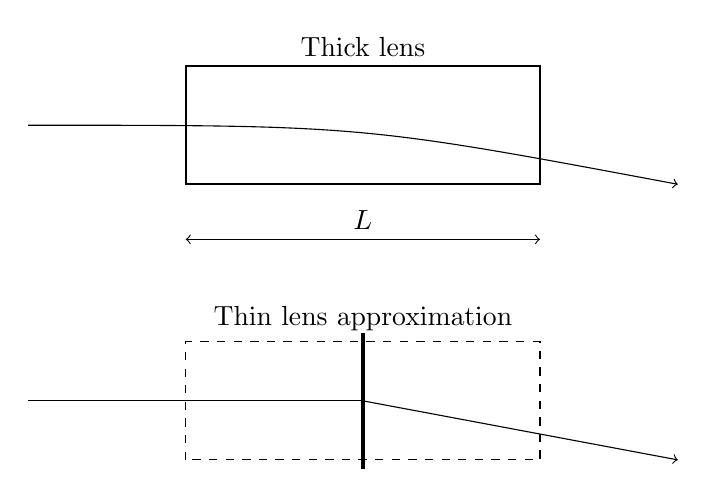
\begin{tikzpicture}
%    \draw[black,thin] (0.0,0.0) grid (16.0,9.0);

    % thick lens 
    \draw[thick] (6.0,4.5) rectangle (10.5,6.0);
    \draw[->] (4.0,5.25) .. controls (8.25,5.25) .. (12.25,4.5);
    \node [rotate=0]  at (8.25,6.25)    {Thick lens};


    %  thin lens
    \draw[dashed]      (6.0,1.0) rectangle (10.5,2.5);
    \draw[<->] (6.0,3.8) -- (10.5,3.8);
    \node [rotate=0]  at (8.25,4.05)    {$L$};

    \draw[thick] (8.24,0.9) rectangle (8.26,2.6);
    \draw (4.0,1.75)  -- (8.25,1.75);
    \draw[->] (8.25,1.75) -- (12.25,1.0);
   \node [rotate=0]  at (8.25,2.80)    {Thin lens approximation};


   
  \end{tikzpicture}
  \caption{Schmematic illustration of the thin lens approximation. The transverse bending of a magnet of length $L$ is approximated by a point-like kick the particle receives only at the center of the magnet. Left and right of the magnet center the particle momentum remaines unchanged.}
  \label{pic:thinlens}
\end{figure}









The analytical treatment of the transfer matrices can be significantly simplified if the magnet length $L$ is small compared to $1/KL$. The magnetic bending can then be treated as a point-like transverse kick which is given to the particle at the center of the magnet, while the the particle trajectory at the rest of the magnet remains undisturbed, so behaves like a drift space (see \figref{pic:thinlens}). Mathematically, this thin lens approximation~\cite{CERN-SL-95-12} corresponds to the limit
\begin{align}
  L \rightarrow 0 \quad \text{with} \quad K \, L = \text{const.} 
\end{align} 
The transfer matrix for a quadrupole magnet simplifies in the thin lens approximation to:
\begin{align}
  \mathcal{M}_{Q,f/d} = \begin{pmatrix}  1 & L \\   KL & 1  \end{pmatrix} \, ,
\end{align}
which is equivalent to the transfer matrix of a thin optical lens with focal length $f=\frac{1}{KL}$.
%
\subsubsection{Periodic Solution and Betatron Motion}
In circular accelerators the quantity $K(s)$ is a periodic quantity with period length $C$:
\begin{align}
K(s) = K(s+C) .
\end{align}
The equation of motion (\ref{eq:hill1}) with periodic $K(s)$ is the Hill differential equation~\cite{wiedemann1999particle}.
The solution of Hill's equation is a quasi-harmonic oscillation 
\begin{align}
x(s) = \sqrt{\tilde{\epsilon}} \, \sqrt{\beta_x(s)} \, \cos \left( \psi(s) + \phi \right) \, , \label{eq:betatron_oscillation}
\end{align}
where $\tilde{\epsilon}$ and $\phi$ are mathematically the integration constants and represent the initial conditions of the particle. The function $\beta_x(s)$ is a periodic function with period $C$, referred to as the betatron function. It is purely defined by the magnetic lattice in the accelerator. 

It defines the maximum local amplitude at a given location. The quantity $\psi(s)$ is the phase of the betatron oscillation defined by
\begin{align}
\psi(s) = \int_0^s \frac{\mathrm{d}s}{\beta(s)} \, .
\end{align}
The total number of betatron oscillations over one turn is the machine tune
%
\begin{align}
  Q = \frac{1}{2 \pi} \int_0^C \frac{\mathrm{d}s}{\beta(s)} \, .
\end{align}
%
%
From \eqref{eq:betatron_oscillation} it can be deduced that $\tilde{\epsilon}$ is a constant of motion\footnote{Note that $\tilde{\epsilon}$ remains constant only if the forces acting on the particle are purely conservative.}, mathematically the Courant-Snyder invariant, for the individual particle:
\begin{align}
\tilde{\epsilon} = \gamma(s) \, x'(s) + 2 \, \alpha(s) \, x(s) \, x'(s) + \beta(s) \, x'^2 (s) \, . \label{eq:parameric_ellipse}
\end{align}
The quantities $\beta(s)$, $\alpha(s)$ and $\gamma(s)$ are the Twiss parameters~\cite{wiedemann1999particle}. They are defined by the beam lattice in the machine. The time derivative of the betatron function $\beta_x(s)$ defines the two other Twiss parameters as:
\begin{align}
\alpha(s) = - \frac{1}{2} \beta'(s) \quad \quad \gamma(s) = \frac{1+\alpha(s)^2}{\beta(s)} \, .
\end{align}

The evolution of an initial set $(\alpha_{x,0},\beta_{x,0},\gamma_{x,0})$ of Twiss parameters in the accelerator depends on the lattice elements and is, equivalent to the transformation of the particle coordinates in \eqref{eq:transfer_matrix}, described by their transfer matrices as follows:
\begin{align}
  \beta_x(s) = C_x^2 \, \beta_{x,0} -2 \, S_x^2 \, C_x^2 \, \alpha_{x,0} + S_x^2 \, \gamma_{x,0} \, .
\end{align}


The expression in \eqref{eq:parameric_ellipse} is the parametric representation of an ellipse in $x,x'$ enclosing a phase space volume of $\pi \tilde{\epsilon}$. Shape and orientation of the phase space ellipse are changing as a function of the the Twiss parameters, but the volume in phase space enclosed by the ellipse remains unchanged (see \figref{fig:phasespace_transformation}). Following \eqref{eq:betatron_oscillation}, the largest possible amplitude in $x$ and $x'$ the particle can reach yields:
%
\begin{align}
  x_\text{max} = \sqrt{\tilde{\epsilon} \, \beta_x(s)} \quad \text{and} \quad x_\text{max}' = - \alpha_x (s) \, \sqrt{\frac{\tilde{\epsilon}}{\beta_x(s)}}
\end{align}

The phase space volume $\tilde{\epsilon}$ is thus related to the peak amplitude of the betatron oscillation for a given $\beta$-function. If many particles compose the beam, the r.m.s. value of the individual $\tilde{\epsilon}$ is referred to as the emittance, which is directly related to the r.m.s. beam size $\sigma_x(s)$:
%
\begin{align}
  \sigma_x (s) = \sqrt{\epsilon_x \, \beta_x} \quad \text{with} \quad \epsilon_x = \langle \tilde{\epsilon_x} \rangle_{\text{rms}} \, .
\end{align}
%
The emittance is a measure for the beam quality and should be as small as possible. It is related to the transverse particle motion, which is reduced due to the relativistic time dilatation. Therefore, the beam emittance decreases proportionally to $\frac{1}{\beta \, \gamma}$ which is known as adiabatic damping. The normalized emittance is defined as 
%
\begin{align}
  \epsilon_N = \epsilon \, \beta \gamma \, ,
\end{align}
and remains constant for all particle energies, assuming that, besides the acceleration, only conservative forces  act on the beam. The emittance is measured in $\mu$m rad.



\begin{figure}[b]  
    \centering
    \includegraphics[width=1\textwidth]{pictures/16021801.pdf}
    \caption{Individual particle trajectories in a periodic quadrupole lattice. The individual betatron amplitude depends on the betatron phase of each particle. The r.m.s. beam envelope is defined by the $\beta$-function and the r.m.s. beam emittance $\epsilon$.}  
    \label{pic:16021801}
    %/home/phermes/Dropbox/PhD/pictures/160217_beam_enveloppe/enveloppe.pdf
\end{figure}


\subsubsection{Solution of the inhomogeneous Equation of Motion}


The solution of the inhomogenious equation of motion \eqref{eq:hill1} is given as
%
\begin{align}
  x(s) = x_h(s) + x_i(s) \, , \label{eq:inhsol}
\end{align}
%
where $x_h(s)$ is the solution of the homogeneous equation shown in \eqref{eq:general_solution} and $x_i$ is one particular solution of the inhomogeneous equation, for example
%
\begin{align}
  x_i(s) = \bar{D}_x(s) \, \delta \, .
\end{align}
%
The dispersion function $\bar{D}_x(s)$ is a periodic function in $s$ with period length $C$, depending on the magnetic elements in the entire ring. It is defined as
%
\begin{align}
  \bar{D}_x (s) = - \frac{\beta_x(s)}{2 \, \sin (\pi \, Q_x)} \, \int_{s_0}^{s_0+C} \, h_x(\tilde{s}) \, \sqrt{\beta(\tilde{s})} \, \cos \left[ 2 \pi \, \left( \psi(\tilde{s}) - \psi(s_0) - \frac{Q_x}{s} \right) \right] \, \mathrm{d} \tilde{s} \, .
\end{align}

In order to be coherent with the definition in the simulation tools used, in the following the dispersion function will be expressed in terms of $D_x(s)$, defined as
%
\begin{align}
  D_x(s) = -\bar{D}_x(s) \, .
\end{align}
%
As shown in \eqref{eq:inhsol}, the dispersion function relates the momentum offset of the particle to an additional transverse amplitude. It thus quantifies the particle deviation due to dispersive effects. Note that this mathematical description represents a linear approximation and higher order dispersive effects are not taken into account. For particles with large momentum offsets, a more accurate description is given by a fully symplectic transformation which can be derived from the accelerator Hamiltonian (see \chapref{chap:hamiltonian}). 



\subsection{Longitudinal Particle Dynamics}

\input{pictures/cavity.tex}

The beams circulating in a high energy synchrotron are bunched, thus there is no continuous current of beam particles through the beam pipe. Rather, dedicated longitudinal slots are assigned for a given number of particle bunches which are populated with the beam particles. The longitudinal bunch spacing and therefore the maximum number of circulating bunches is determined by the accelerating RF cavities which keep the particles in phase at constant energy and accelerate them to the top energy~\cite{wiedemann1999particle}. 

An accelerating cavity operated at an angular frequency $\omega$ provides an electric field given by~\cite{}:
\begin{align}
  V(t) = V_0 \, \sin (\omega \, t) \, .
\end{align}
Using the revolution time $T_S$ of the synchronous particle, the frequency of the RF cavity can be expressed as
\begin{align}
  \omega = h \, \frac{2 \, \pi}{T_S} \, ,
\end{align}
where $\omega$ is chosen such that $h$ is an integer, the harmonic number. The latter condition assures that the synchronous particle is in phase with the RF voltage, such that the energetic kick it receives remains constant. A real particle is not in phase with the RF cavity, but arrives with a certain phase offset
%



